\documentclass[11pt,twocolumn]{article}

\usepackage{hyperref}
\usepackage{graphicx}
% \usepackage{fullpage}

\linespread{1.2}
\setlength{\parskip}{1ex plus 0.5ex minus 0.2ex}

\begin{document}

\title{CSE 549\\Computational Biology -- Progress Report\\Genome Compression}
\author{Pragya Pande \and Dhruv Matani}
\date{\today}

\maketitle

\vspace{0.5in}

\section*{Approach adopted}

We started off with the following approach:
\begin{enumerate}

\item $Ref_i$ is our reference chromosome and $Victim_i$ is the
  chromosome to be compressed

\item For each chromosome pair $Ref_i$ and $Victim_i$, build a \textit{suffix
  array}\footnote{This is done using Manber \& Myers $O(n\log{n})$
  suffix array construction algorithm, which allows us to compute the
  \textit{Longest common Prefix} of 2 adjacent suffixes in
  $O(\log{n})$ time} from the string $Ref_i\#Victim_i\$$

\item Find the longest substring for every string starting at every
  index in $Victim_i$ that is present in $Ref_i$\footnote{This is
    similar to the mid-term question}

\item Now that we have all the ranges that the \textit{victim}
  chromosome can be covered by, we find the least number of ranges
  that can completely cover the \textit{victim}. This can be done in
  $O(n\log{n})$ using \textit{Dynamic Programming} and \textit{Segment
    Trees} as an online \textit{Range Minimum Query} data
  structure. The problem of finding the minimal number of completely
  covering sub-ranges exhibits optimal substructure. i.e. A solution
  for the range $(i..n)$ can be constructed using the solution to the
  ranges $(i+1..n), (i+2..n), (i+3..n), \ldots{}, (i+k-1..n)$, where
  $k$ is the length of the range starting at index $i$.

\end{enumerate}

\begin{figure}
  \begin{center}
    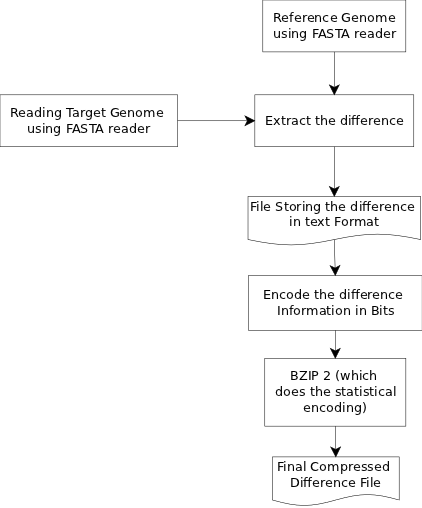
\includegraphics[height=3.4in]{figures/GenomeCompressionFlow.png}
    \caption{The flow of Genome Compression}
    \label{fig:genomecompressionflow}
  \end{center}
\end {figure}

The total running time of our algorithm is $O(n\log{n})$, where $n$ is
the length of the 2 concatenated chromosomes.

After running our algorithm on 2 chromosomes, we found that the
average length of an overlapping substring is about $10$ and not $250$
as we had expected (since 2 human genomes are considered to differ in
only about 1 of 1000 bases).

The 2 chromosomes we used were from \textit{hg18}, which is
\textit{build 36.1} on \textit{http://ncbi.nih.gov/} and \textit{build
  36.3} on the same site.

Any insight into why this is happening would be great since one of the
assumptions that we were banking on has been falsified.

When we compared a chromosome with itself, we got back a single range
covering the entire genome. In another experiment, we compared a
chromosome with itself, but with a few mutations, and we got back the
correct expected small number of long ranges.

In hind-sight, we think we could have saved some time by running some
basic tests which ran a crude algorithm to find the average length of
overlaps between genomes.

We have also started work on an encoding scheme that efficiently packs
range data into a tight binary representation. There are 3 types of
cases that we wanted to handle:

\begin{enumerate}

\item \textit{Ranges:} A range specifies an $(offset, length)$ into
  the reference chromosome that should be copied to the output to
  reconstruct the victim chromosome. Each range looks like this:
\begin{verbatim}
6155526 170
\end{verbatim}
Which means that we should print $170$ characters from offset
$6155526$ in the reference chromosome to the current output.

\item \textit{Single character:} A single character is represented as
  the character itself. e.g.
\begin{verbatim}
A
\end{verbatim}

\item \textit{Repeated character:} A repeated character is represented
  by the character followed by the number of times it is
  repeated. e.g.
\begin{verbatim}
C 33
\end{verbatim}

\end{enumerate}

To represent these types of operations in binary, we represent a
single character as a 4-bit entity, whose MSB\footnote{Most
  Significant Bit is reset (0)}. The remaining 3 bits represent one of
\textit{A, C, G, T, or N}.

A character repeat is encoded in a 32-bit entity where the first 2
bits are \textit{00}. The next 3 bits are the encoding of the
character itself (similar to the single character encoding above). The
remaining 27 bits hold the count of run.

A range is represented by a 48-bit entity with the first 2 significant
bits set to \textit{01}. The next 14 bits hold the length of the run
and the last 32 bits hold the offset of this run in the reference
chromosome.

\section*{Shortcomings}

The approach we have used doesn't seem to work since the average
length of a run that matches some run in the reference chromosome is
just 10 (v/s the 250 that we were expecting on average). This seems to
go against our initial intuition of 2 human genomes being 99\% similar
in their bases.

We would like to talk to you about this.

\section*{We we had planned}

\begin{enumerate}

\item Find reversals of a string in the reference genome

\item Find complements of a string in the reference genome

\item Find reverse complements of a string in the reference genome

\item Convert ranges less than a certain threshold value $k$ to a
  single character. For example, if we have a range of length 4, then
  it would use up 48-bits on disk, whereas if we store them as single
  characters, it would use $4*3 = 12$-bits on disk.

\item If we have 3 ranges such that the center range has a length less
  than a certain threshold $k$ and its length is the same as the
  difference in the start and end offsets of the last and first ranges
  respectively, then we can encode all three ranges as a single range
  and add the substituted characters as specially encoded \textit{back
    substitutions}.

\end{enumerate}

\section*{Plan-B}

Plan-B involves directly using the SNP file containing the
\textit{insertions, deletions, \& substitutions} needed to construct a
chromosome with respect to the reference chromosome in the
\textit{hg18} genome.

After investigating the
DNAZip\footnote{\textit{http://www.ics.uci.edu/~dnazip/index.html}}
code, it seems that there is scope for reducing the size of the stored
structures on disk by applying huffman encoding on some of the
internal structures that are being written out to disk.

We shall further investigate the scope of this Plan.

\clearpage


\end{document}
